\documentclass [a4paper,10pt,oneside] {article}
\usepackage[colorlinks,linkcolor=gray,anchorcolor=black,citecolor=blue,filecolor=cyan,menucolor=gray]{hyperref}
\usepackage{hyperref}
\usepackage{xeCJK}
\usepackage{graphics}
\usepackage{epsfig}
\usepackage{enumerate} %枚举宏包
\usepackage{listings}
\usepackage{geometry}
\usepackage{indentfirst}
\usepackage{xcolor}
\punctstyle{kaiming}
\usepackage{booktabs}
\usepackage{multirow}
\usepackage{tikz}
\definecolor{mygray}{rgb}{0.3,0.3,0.3}
\definecolor{codegreen}{rgb}{0.8,0.8,0.8}
\vspace{50pt}%调整表格行高
\linespread{1.30}%行间距
\geometry{a4paper,left=2cm,right=2cm,top=1cm,bottom=1.5cm}
\setcounter{secnumdepth}{4}
\setcounter{tocdepth}{4}


%设置字体
%\setmainfont{STKAITI.TTF}
%\setmainfont{Noto Sans CJK JP Thin}
\setmainfont{Ubuntu}
%\setCJKmainfont{SimSun} % 语义和语法同fontspec
%\setCJKsansfont{SimHei}
%\setCJKmonofont{SimSun}


\makeatletter



\lstset{
	numbers=left,
	numberstyle=\tiny,
	basicstyle=\scriptsize,
	backgroundcolor= \color{gray},
	keywordstyle=\color{blue!70},
	breaklines=true,
	breakautoindent=true,
	breakindent=4em,
	commentstyle=\color{codegreen},
	frame=shadowbox,
	escapeinside=``,
	tabsize=4,
	framextopmargin=1pt,framexbottommargin=1pt,abovecaptionskip=-1pt,belowcaptionskip=1pt,
  xleftmargin=3em,xrightmargin=3em,
	language=C
}
\begin{document}


\title{\textbf{Body Area Network }\\ % Title
 Design For Test}  % Subtitle

\author{\textsc{haobo.gao} % Author
\\{\textbf{Foxconn ZZDC}}} % Institution

\date{\today} % Date
\maketitle

\pagenumbering{roman}
\tableofcontents
\pagenumbering{arabic}
\section{Overview}







图 \ref{Overview} 是BAN(Body Area Network)的构想图,假设了三个设备在BAN 上的情况。



\begin{figure*}[htbp]
\begin{center}
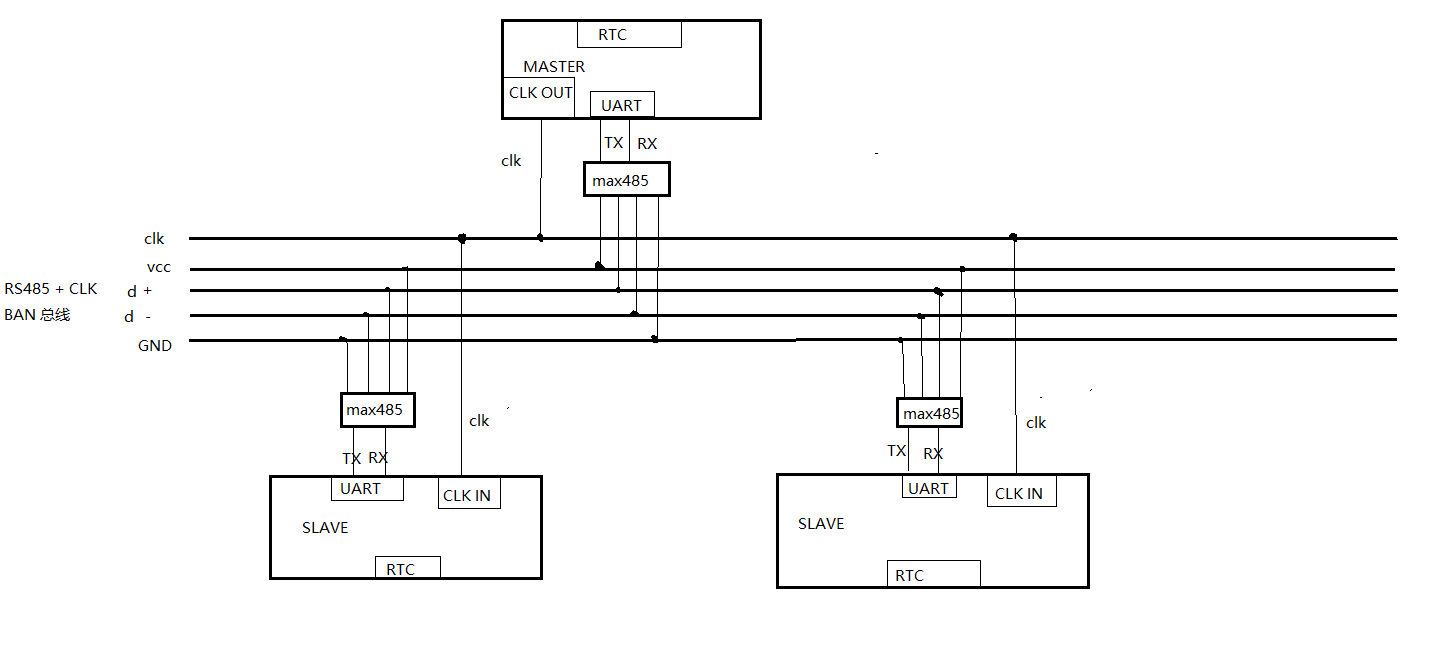
\includegraphics[width=15cm]{img/overview}
\caption{BAN }
\label{Overview}
\end{center}
\vspace{-0.5em}
\end{figure*}


下面是对于这个构想图模块的解释。




\subsection{CLK}

这个是BAN 的时钟线,时钟信号由 MASTER 产生,挂载在总线上的从设备会去监测捕获这条时钟线
的上升沿。时钟的产生方式是:定时器产生的PWM。如图\ref{timer} \tikz \fill[red] (1ex,1ex) circle (1ex);

\begin{figure*}[htbp]
\begin{center}
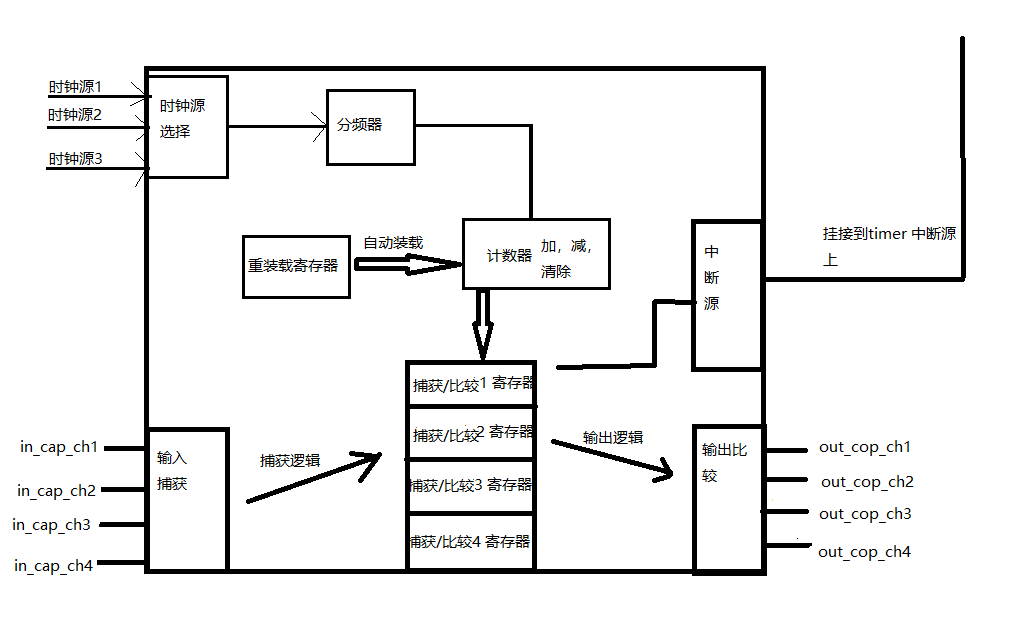
\includegraphics[width=15cm]{img/timer}
\caption{PWM}
\label{timer}
\end{center}
\vspace{-0.5em}
\end{figure*}






\subsection{RTC}

大多数时候RTC 其实是一个独立供电的(纽扣电池),有特殊寄存器(年月日)的 timer。

在本次测试中,由于时间和硬件资源的原因,每一个设备都会使用一个精准定时器用于精确
定时,维护一个unsigned long long 类型的时间戳。

\begin{figure*}[htbp]
  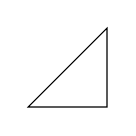
\begin{tikzpicture}
\draw (0,0) -- (1,0) -- (1,1) -- cycle;
  \end{tikzpicture}
\caption{Do not forget!}
\end{figure*}



\subsection{UART}




\subsection{测试例程逻辑}



主从机代码均有 cmd\_handle 用于相应来自于串口的命令。


这些命令有

\subsubsection{begin 命令}

 begin 当板子接收到来自于串口的begin 字串的时候:

 \begin{itemize}
   \item 1. 会去从零开始计算时间戳,并开始PWM 产生(主机)或者 捕获(从机),这点主机从机都一样。

   \item 主机接收到begin 命令后, 会去给从机发送begin 字符串,然后 再开始 1 。

   \item

 \end{itemize}

\section{Introduce}



\subsection{同步流程}



\subsection{结语}
\include{chap/other}

\end{document}
